\documentclass[10pt,a4paper]{article}
\usepackage[margin=17mm]{geometry}
\usepackage[T1]{fontenc}
\usepackage{lmodern,amsmath,graphicx,xcolor,booktabs}
\usepackage[hidelinks]{hyperref}
\usepackage{fancyhdr}
\pagestyle{fancy}\fancyhf{}\fancyfoot[L]{\small AIAA3201 / Lab 06}\fancyfoot[R]{\small\thepage}
\renewcommand{\headrulewidth}{0pt}
\setlength{\parindent}{0pt}\setlength{\parskip}{5pt}
\definecolor{navy}{HTML}{172A46}
\newcommand{\sectiontitle}[1]{\par\vspace{5pt}{\large\bfseries\color{navy}#1}\par}
\newcommand{\captiontext}[1]{{\footnotesize\color{black!65}#1\par}}
\begin{document}
{\LARGE\bfseries\color{navy}Building and Inspecting Neural Networks}\par
\smallskip
{\small AIAA3201 Lab 06 \quad | \quad 19 October 2026 \quad | \quad Conda: \texttt{aiaa3201}, CPU}

\sectiontitle{Part 1: XOR convergence}
With the original settings (NumPy seed 42, two hidden units, learning rate 0.5), the network first meets
\(\max_i |\hat y_i-y_i|\leq 0.1\) after \textbf{8,304 parameter updates}.
In input order \((0,0),(0,1),(1,0),(1,1)\), its predictions are
\[
\hat y=[0.090604,\ 0.900009,\ 0.900158,\ 0.080664],
\qquad E=\tfrac12\operatorname{mean}(\hat y-y)^2=0.00433532.
\]
The previous update does not meet the tolerance. The first five printed losses decrease from
0.143150 to 0.137942. These table rows use predictions \emph{before} each update;
after five updates the loss is 0.136844.

If convergence stayed slow, I would tune the learning rate, try more hidden units and different
random seeds, and inspect gradient magnitudes. A Sigmoid derivative is at most 0.25 and approaches
zero in saturation, so gradients can be attenuated. Alternative hidden activations and suitable
initialization may help. These are proposed remedies, not additional measured results.

\begin{center}
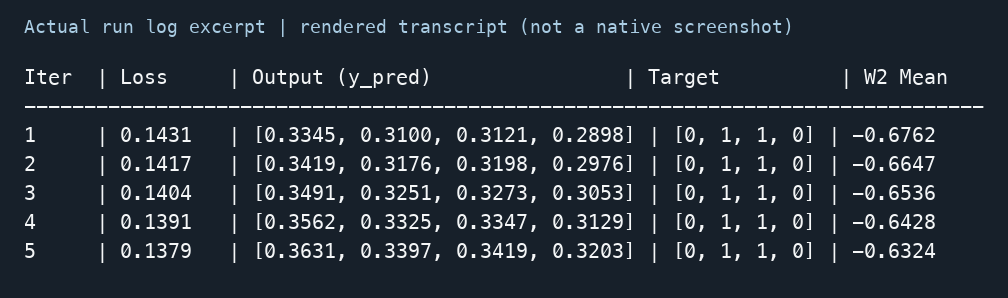
\includegraphics[width=\linewidth]{screenshots/part1_run_transcript.png}
\end{center}
\captiontext{Figure 1. First five iterations from \texttt{logs/main\_run.txt}; actual output rendered as an image.}

\sectiontitle{Part 2: Sigmoid versus ReLU}
Both \(2\!\to\!16\!\to\!16\!\to\!1\) networks use identical initial linear parameters (seed 42), the same
1,000 concentric-circle samples, full-batch SGD (learning rate 0.05), BCE, and 1,000 epochs.
The output activation is Sigmoid in both models.
\begin{center}
\begin{tabular}{lrrr}
\toprule
Hidden activation & Initial BCE & Final BCE & Training accuracy\\
\midrule
Sigmoid & 0.735396 & 0.693194 & 29.30\%\\
ReLU & 0.701004 & 0.138952 & 100.00\%\\
\bottomrule
\end{tabular}
\end{center}
Final metrics are evaluated after update 1,000; the plotted curve records the losses before each update.
Here ReLU learns the circular separation much faster. Repeated Sigmoid derivatives attenuate
gradients, whereas active ReLU units have derivative 1 and support stronger gradient flow.
Sigmoid stays near the uninformative BCE value \(\ln 2\), with probabilities near 0.5 and a poor
boundary. This comparison is specific to this initialization and training setup; ReLU does not
always win, and inactive ReLU units can receive zero gradients. These are training results,
not held-out generalization results.

\newpage
{\LARGE\bfseries\color{navy}Verification and experimental evidence}\par
\begin{center}
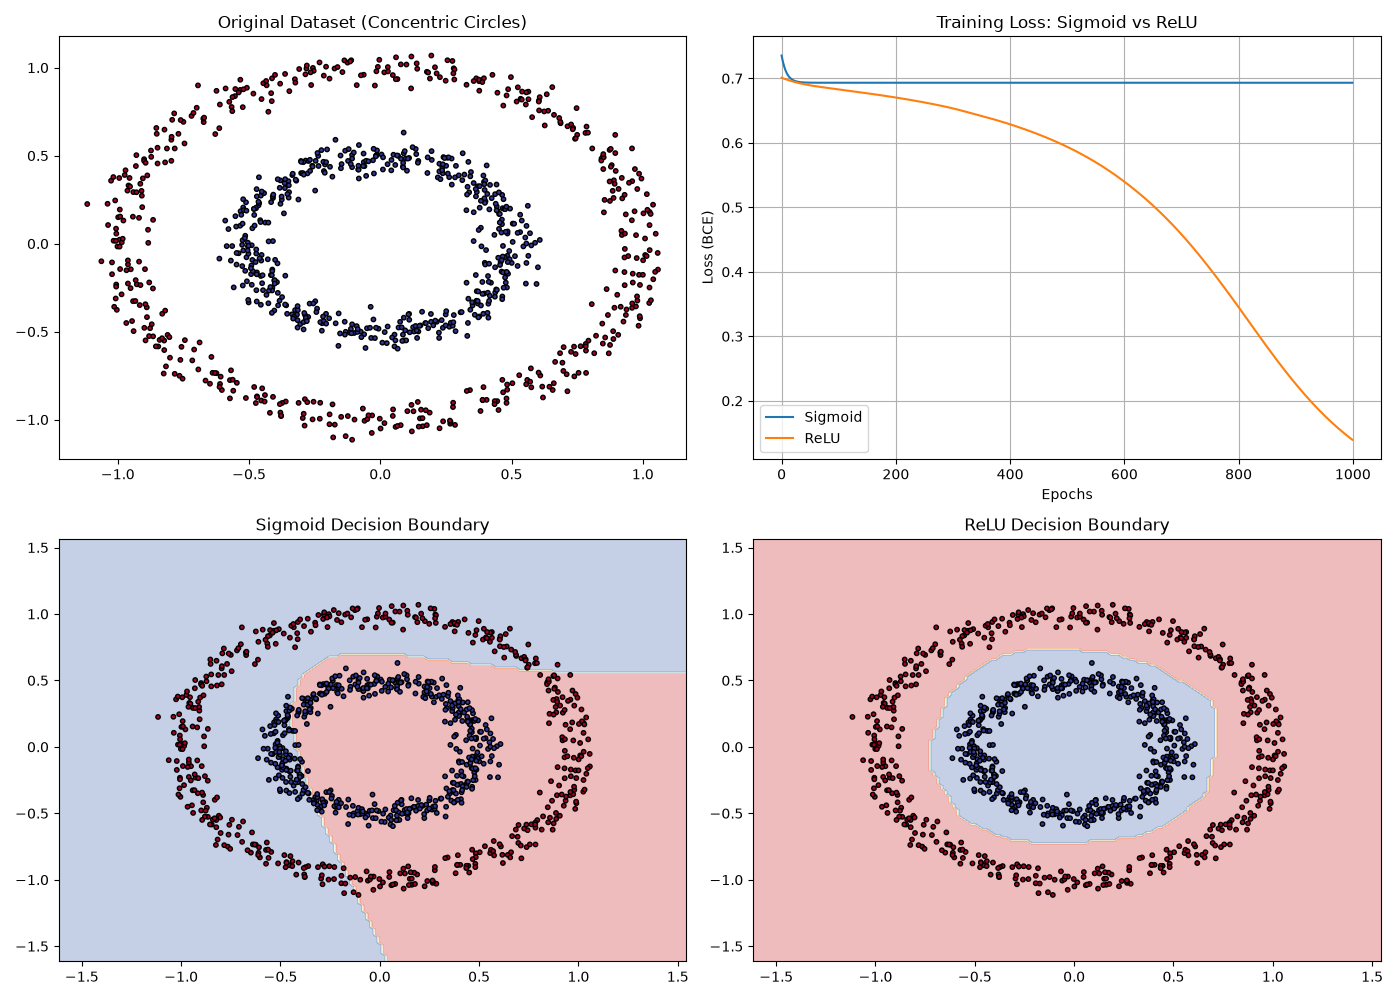
\includegraphics[width=0.62\linewidth]{plots/activation_comprehensive_analysis.png}
\end{center}
\captiontext{Figure 2. Required four-panel plot generated by the complete \texttt{python main.py} run.}

\sectiontitle{Part 3: Independent calculation and PyTorch verification}
Seed 42 selects \(N=32,C_{\rm in}=1,C_{\rm out}=64,F=5,s=1,P=1\). With dilation 1:
\[
H_{\rm out}=W_{\rm out}=\left\lfloor\frac{32+2(1)-5}{1}\right\rfloor+1=30,
\qquad \#\theta=64\,(1\cdot5\cdot5+1)=1,664.
\]
The bias is included; expected tensor shape: \([1,64,30,30]\). Settings were generated with the
unimplemented script; the independent calculation preceded implementation and PyTorch verification.
\begin{center}
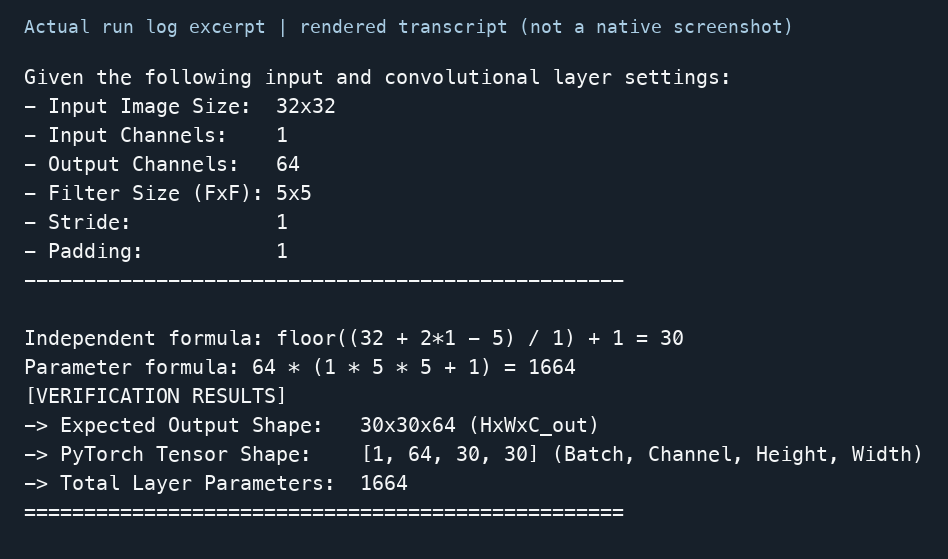
\includegraphics[width=0.90\linewidth]{screenshots/part3_run_transcript.png}
\end{center}
\captiontext{Figure 3. Settings and verification results excerpted from the same complete run log.}

\sectiontitle{Requirements and evidence provenance}
{\footnotesize
The page and README checklists agree. Extra evidence requested in the README task text and slide 5
comprises CNN calculations and terminal images for Parts 1 and 3. Native Terminal/Codex screenshot
access was blocked by the system. Figures 1 and 3 are labelled renderings of actual output,
\textbf{not native terminal screenshots}. Original text logs and PNG transcripts are included.

Validation: finite-difference NumPy gradient max absolute error \(1.68\times10^{-11}\);
five-round loss decreases; CNN tensor shape and parameter count match both formulas.
Versions are recorded in \texttt{requirements.txt} and \texttt{logs/environment.txt}.
}
\end{document}
